\chapter{电场与磁场中的带电粒子}\label{ch:b1:charged-particles}

在\cref{ch:b1:transient-regimes}中描绘波形的示波器内部，
一束电子在两极板间电压的作用下扫过屏幕；
在质谱仪的磁铁内部，两种同位素的离子
因其中一种比另一种重百分之八，相隔数毫米而被分开；
在医院的回旋加速器内，质子向外盘旋，
历经两百圈后以光速的三分之一射出，
用来灼烧肿瘤。三者遵循同一动力学：电荷在
均匀的电场或磁场中运动，并服从牛顿定律。
本章由此推导——电场中的抛物线，磁场中的圆周与
螺旋线——并将其转化为用于
分选、加速和测量带电粒子的仪器。

\begin{omfigure}
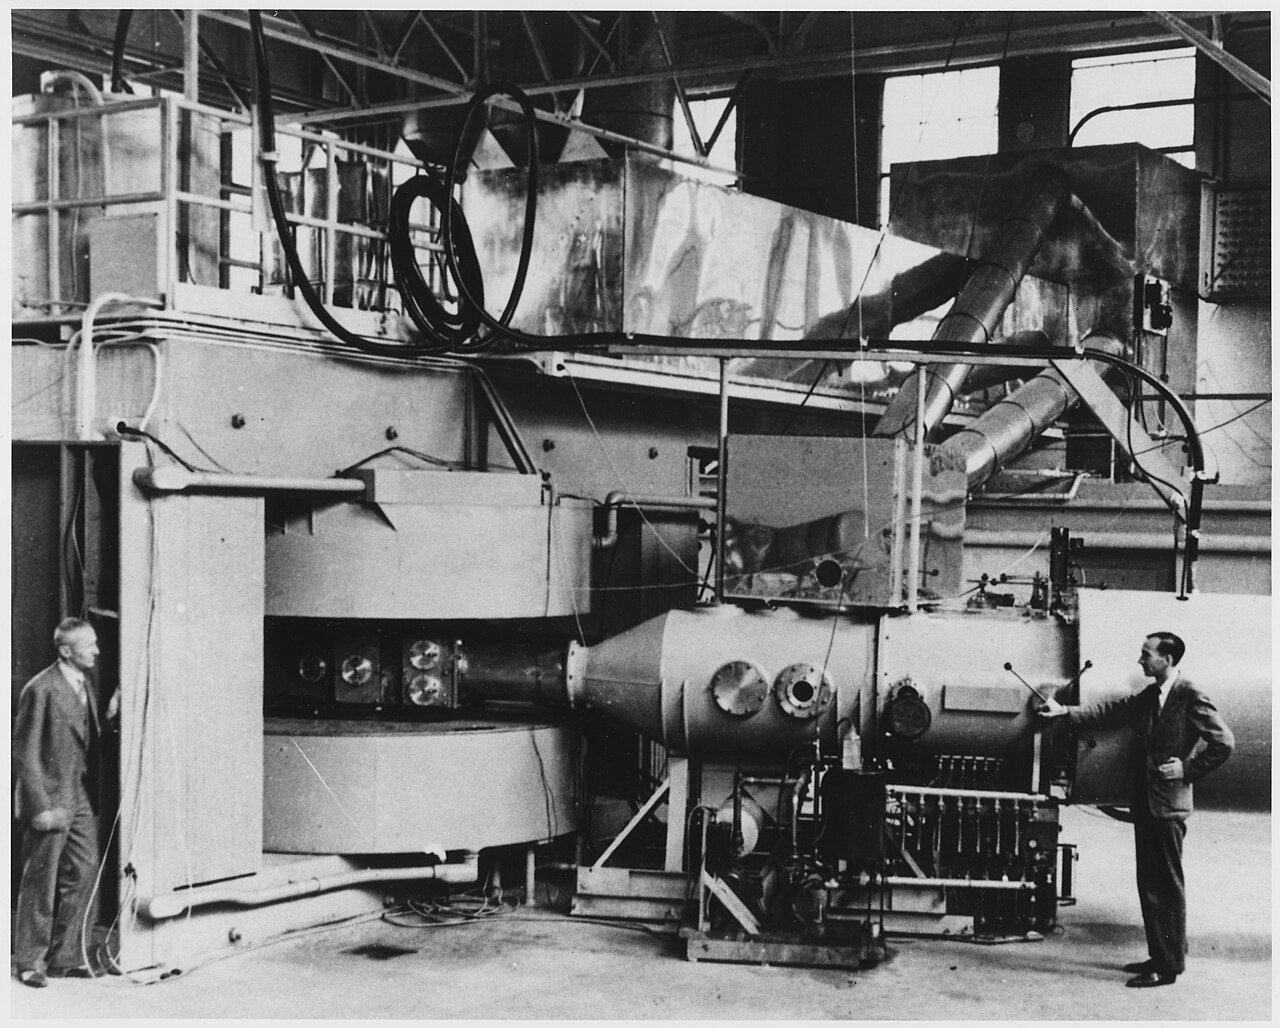
\includegraphics[width=0.60\linewidth]{images/book3/cyclotron-berkeley-60inch.jpg}

{\small 伯克利的劳伦斯 60 英寸回旋加速器，1939 年（美国能源部）：质子在磁铁两极之间每转一圈被加速两次，向外盘旋，与周末问题中的情形完全相同。}
\end{omfigure}

\section{洛伦兹力}

\begin{definition}[洛伦兹力]\label{def:b1:charged-particles:lorentz}
\index{洛伦兹力}\index{电场}\index{磁场}
电荷为 $q$、以速度 $\vect v$ 运动的粒子，在电场
$\vect E$ 与磁场 $\vect B$ 中，所受的力为
\[
\vect F = q\big(\vect E + \vect v\wedge\vect B\big) .
\]
电场力沿 $\vect E$ 方向（若 $q < 0$ 则反向），
与运动无关；磁场力同时垂直于
$\vect v$ 与 $\vect B$，大小与速率成正比，且对
静止粒子为零。单位：$\vect E$ 以 \unit{V/m}（或 \unit{N/C}），$\vect B$
以特斯拉（\unit{T}）计：$\qty{1}{T} = \qty{1}{N/(A.m)}$。
\end{definition}

\begin{proposition}[洛伦兹力的功]\label{prop:b1:charged-particles:work}
磁场力不做功：其功率 $q(\vect v\wedge\vect B)\cdot\vect v$
为零，因此仅有磁场时只改变速度的方向，
从不改变速率或动能。电场力的功率为
$q\vect E\cdot\vect v$，两点间电场力所做的功为 $q(V_A - V_B) =
qU_{AB}$（见\cref{ch:b1:potential-capacitors}）：电荷为 $q$ 的粒子
穿过电压 $U$ 时获得动能 $\abs{qU}$。
\end{proposition}

\begin{proof}
$\vect v\wedge\vect B \perp \vect v$。静电场由电势导出，
即 $\vect E = -\overrightarrow{\operatorname{grad}}V$，因此 $q\vect E$
是保守力，其势能为 $E_p = qV$。
\end{proof}

\begin{definition}[电子伏特]\label{def:b1:charged-particles:eV}
\index{电子伏特}
\emph{电子伏特}是一个元电荷
穿过一伏特电压时获得的动能：$\qty{1}{eV} = \qty{1.60e-19}{J}$。
化学过程约为几 eV，X 射线管约为数十 keV，核物理为 MeV 量级，
粒子物理为 GeV 与 TeV 量级。
\end{definition}

\begin{remark}[为何忽略重力]\label{rem:b1:charged-particles:gravity}
对于处在 \qty{1}{kV/m} 电场中的电子——这是一个适中的实验室数值——
电场力为 $eE = \qty{1.6e-16}{N}$，与重力
$mg = \qty{9e-30}{N}$ 相比小 $10^{13}$ 倍。
本章所有计算均略去重力，无须多加考虑。（相对论
极限则另当别论：下述公式在
$\tfrac12 mv^2 \ll mc^2$ 条件下成立，即对电子低于约 \qty{50}{keV}，
对质子低于约 \qty{100}{MeV}；见本科三年级分册。）
\end{remark}

\section{均匀电场}

\begin{proposition}[加速与偏转]\label{prop:b1:charged-particles:efield}
\index{加速电压}
在均匀电场 $\vect E$ 中，加速度 $\vect a = q\vect E/m$
为常矢量：运动与抛体运动相同，仅以 $q\vect E/m$ 代替
$\vect g$。
\begin{itemize}
  \item 自静止释放并经电压 $U$ 加速，
        粒子达到 $v = \sqrt{2\abs{qU}/m}$。
  \item 以速率 $v_0$ 沿 $x$ 方向进入长为 $L$ 的区域，
        其中 $\vect E = E\vect e_y$，粒子沿抛物线 $y = (qE/2mv_0^2)x^2$ 运动，
        离开时偏转角为 $\alpha$，且 $\tan\alpha =
        qEL/mv_0^2$，仿佛它是沿直线从
        极板中央射来的。
\end{itemize}
\end{proposition}

\begin{proof}
能量：$\tfrac12 mv^2 = \abs{qU}$。偏转：$x = v_0t$，$y =
\tfrac12(qE/m)t^2$；出口处 $\dd y/\dd x = (qE/m)(x/v_0^2)$ 在
$L$ 处取值；出口处的切线 $y = (qEL/mv_0^2)(x - L/2)$ 与
轴交于 $x = L/2$ 处。
\end{proof}

\begin{omfigure}
\begin{tikzpicture}[font=\small, x=1cm, y=1cm]
  \draw[thick] (0,1.1) -- (3.6,1.1); \draw[thick] (0,-1.1) -- (3.6,-1.1);
  \node[above] at (1.8,1.1) {$-$}; \node[below] at (1.8,-1.1) {$+$};
  \draw[-Stealth, omDef] (1.2,-0.85) -- (1.2,0.85) node[midway, left] {$\vect E$};
  \draw[-Stealth, omThm, thick] (-1.6,0) -- (0,0) node[pos=0.3, above] {$v_0$};
  \draw[omThm, thick, domain=0:3.6, samples=50] plot (\x, {-0.06*\x*\x});
  % exit at x=3.6: y=-0.778, slope=-0.432
  \draw[-Stealth, omThm, thick] (3.6,-0.778) -- (6.4,{-0.778-0.432*2.8});
  \draw[dashed, omExo] (1.8,0) -- (6.4,{-0.432*4.6});
  \draw[dashed] (-0.2,0) -- (6.6,0);
  \draw (5.0,0) arc (0:-23.4:1.4); \node at (5.4,-0.35) {$\alpha$};
  \draw[thick] (7.0,-2.4) -- (7.0,1.2); \node[above] at (7.0,1.2) {屏幕};
  \fill[omThm] (7.0,{-0.778-0.432*3.4}) circle (1.8pt);
  \draw[Stealth-Stealth] (0,1.5) -- (3.6,1.5) node[midway, above] {$L$};
  \node[omExo, font=\footnotesize, below] at (1.8,-0.05) {$L/2$};
  \fill (1.8,0) circle (1.2pt);
\end{tikzpicture}

{\small 静电偏转：在极板之间，电子（此处
$q < 0$，向正极板偏转）沿抛物线运动；越出极板后
它沿直线飞行，仿佛从极板中点射出，
——这便是阴极射线示波管的几何原理。}
\end{omfigure}

\begin{example}[示波管]\label{ex:b1:charged-particles:crt}
电子经 $U_0 = \qty{2.0}{kV}$ 加速（$v_0 = \qty{2.65e7}{m/s}$，
约为光速 $c$——尚属非相对论），穿过长 \qty{4.0}{cm} 的极板
间距 \qty{1.0}{cm}、电压 \qty{100}{V}：$E = \qty{1.0e4}{V/m}$，
$\tan\alpha = eEL/mv_0^2 = EL/2U_0 = 0.10$，屏幕位于距极板中心 \qty{30}{cm}
处光点移动 \qty{3.0}{cm}——即每伏 \qty{0.3}{mm}，
示波管的灵敏度，完全由几何结构和
加速电压决定。
\end{example}

\section{匀强磁场}

\begin{theorem}[匀强磁场中的运动]\label{thm:b1:charged-particles:bfield}
\index{回旋运动}\index{拉莫尔半径}\index{回旋频率}\index{螺旋运动}
电荷为 $q$、质量为 $m$ 的粒子，速度 $\vect v_0$ 与
匀强 $\vect B$ 垂直，则粒子以恒定速率 $v_0$ 做圆周运动，
其半径和角频率分别为
\[
R = \frac{mv_0}{\abs q B}, \qquad \omega_c = \frac{\abs q B}{m},
\]
其中\emph{回旋频率} $\omega_c$ 与速率无关；
回转方向取决于 $q$ 的正负。若 $\vect v_0$ 还具有
分量 $v_\parallel$（沿 $\vect B$ 方向），该分量保持不变，
轨迹为\emph{螺旋线}，半径为 $mv_\perp/\abs qB$，螺距为
$2\pi mv_\parallel/\abs qB$，绕场线缠绕。
\end{theorem}

\begin{proof}
力 $q\vect v\wedge\vect B$ 与 $\vect v$、$\vect B$ 均垂直；
速率恒定（不做功），沿 $\vect B$ 方向的分量
不受力。在与 $\vect B$ 垂直的平面内，力的
大小恒为 $\abs qv_\perp B$，且始终与速度垂直，故为
匀速圆周运动（见\cref{thm:b1:point-kinematics:frenet}），有 $mv_\perp^2/R =
\abs qv_\perp B$。于是 $\omega_c = v_\perp/R$，
螺距即为周期 $2\pi m/\abs qB$ 与 $v_\parallel$ 之积。
\end{proof}

\begin{omfigure}
\begin{tikzpicture}[font=\small, x=1cm, y=1cm]
  % circle in a plane, B out of page
  \foreach \x in {-1.8,-0.6,0.6,1.8} \foreach \y in {-1.8,-0.6,0.6,1.8} {\draw (\x,\y) circle (0.07); \fill (\x,\y) circle (0.8pt);}
  \node[omDef, right] at (2.1,2.25) {$\vect B$（垂直纸面向外）};
  \draw[omThm, thick] (0,0) circle (1.3);
  \fill[omThm] (1.3,0) circle (1.6pt);
  \draw[-Stealth, omThm, thick] (1.3,0) -- (1.3,1.1) node[right] {$\vect v$};
  \draw[-Stealth, omDef, thick] (1.3,0) -- (0.3,0) node[below, pos=0.6] {$q\vect v\wedge\vect B$};
  \node[omThm, font=\footnotesize] at (0,-2.3) {$R = \dfrac{mv}{\abs qB}$};
  % helix on the right
  \begin{scope}[xshift=6.5cm]
  \draw[-Stealth, omDef, thick] (-0.4,-2.2) -- (-0.4,2.4) node[above] {$\vect B$};
  \draw[omThm, thick, domain=0:12.57, samples=200, variable=\t] plot ({0.9*cos(deg(\t))+1.0},{0.16*\t-2.0+0.3*sin(deg(\t))});
  \node[omThm, font=\footnotesize, right] at (2.0,-0.2) {螺距 $2\pi mv_\parallel/\abs qB$};
  \end{scope}
\end{tikzpicture}

{\small 左：速度与 $\vect B$ 垂直的电荷
以回旋频率 $\abs qB/m$ 做圆周运动，磁力
提供向心加速度。右：速度另有
沿 $\vect B$ 方向的分量，则绕场线螺旋前进——
即地球磁场中被束缚的电子的运动。}
\end{omfigure}

\begin{example}[数量级]\label{ex:b1:charged-particles:orders}
一个 \qty{1}{keV} 的电子（$v = \qty{1.9e7}{m/s}$）置于 \qty{1}{mT} 的磁场中：
$R = \qty{11}{cm}$，$\omega_c = \qty{1.8e8}{rad/s}$，转一圈
需 \qty{36}{ns}——周期与能量无关，这正是使
回旋加速器得以实现的原因。太阳风中的一个质子（\qty{1}{keV}，
\qty{4.4e5}{m/s}）处于地球磁场 \qty{50}{\micro T} 中：$R = \qty{92}{m}$；
它无法穿越场线，只能沿场线
向两极螺旋运动——这便是极光。
\end{example}

\section{仪器}

\begin{proposition}[速度选择器与质谱仪]\label{prop:b1:charged-particles:spectrometer}
\index{速度选择器}\index{质谱仪}
在相互垂直的匀强电场和匀强磁场 $\vect E \perp \vect B$ 中，粒子
沿与二者都垂直的方向运动时不偏转，当且仅当 $v = E/B$，与其
电荷和质量无关（\emph{速度选择器}）。仅在磁场中，已知速率的
粒子做直径为 $2mv/\abs qB$ 的半圆运动：
测量其直径即可得 $m/q$（\emph{质谱仪}）。离子经电压 $U$ 加速，
再在 $B$ 中偏转，落在
\[
R = \frac{1}{B}\sqrt{\frac{2mU}{\abs q}} :
\]
质量分别为 $m$ 与 $m + \Delta m$ 的两种同位素，分开的距离 $\Delta R \approx
R\,\Delta m/2m$。
\end{proposition}

\begin{proof}
$q\vect E + q\vect v\wedge\vect B = \vect 0$ 要求 $vB = E$，方向须
正确。$R = mv/qB$，$v = \sqrt{2qU/m}$；对
$\ln R = \tfrac12\ln m + \text{常数}$ 取微分。
\end{proof}

\begin{example}[碳同位素]\label{ex:b1:charged-particles:isotopes}
一价的 $^{12}$C 与 $^{13}$C 离子经 \qty{20}{kV} 加速，
后进入 \qty{0.50}{T} 的磁场：$R = \qty{14.1}{cm}$ 与 \qty{14.7}{cm}，
相距 \qty{5.8}{mm}——在探测器上形成两个分开的光斑，二者强度之比
即同位素丰度，是放射性碳测年与
一切同位素分析的基础材料。
\end{example}

\begin{proposition}[回旋加速器]\label{prop:b1:charged-particles:cyclotron}
\index{回旋加速器}
两个中空半圆筒（“D 形盒”）置于匀强 $\vect B$ 中，
两者之间加有频率等于回旋频率的交变电压 $U$：
粒子在每个 D 形盒内做圆周运动（盒内无电场），
每转一周两次穿过缝隙时被加速，每次获得 $\abs qU$ 的能量，并向外螺旋前进，
即 $R \propto v$；在引出半径 $R_{\max}$ 处，粒子的动能
为
\[
E_k = \frac{q^2B^2R_{\max}^2}{2m},
\]
与电压无关，电压只决定回旋的圈数。
\end{proposition}

\begin{proof}
 因为 $\omega_c$ 与速率无关，定频电压
 便能逐圈与粒子保持同步；速率为 $v = \abs qBR/m$，
 其中 $R$ 为轨道半径。
\end{proof}

\begin{omfigure}
\begin{tikzpicture}[font=\small, x=1cm, y=1cm]
  \draw[thick, omDef] (0,0) ++(95:2.4) arc (95:265:2.4);
  \draw[thick, omDef] (0,0) ++(-85:2.4) arc (-85:85:2.4);
  \draw[thick, omDef] (-0.2,2.4) -- (-0.2,-2.4); \draw[thick, omDef] (0.2,2.4) -- (0.2,-2.4);
  \node[omDef] at (-1.6,1.9) {D 形盒}; \node[omDef] at (1.6,1.9) {D 形盒};
  \node[above] at (0,2.5) {$U\cos\omega_ct$};
  \draw[omThm, thick, domain=0:1440, samples=300, variable=\t] plot ({(0.15+0.0011*\t)*cos(\t)},{(0.15+0.0011*\t)*sin(\t)});
  \draw[-Stealth, omThm, thick] ({(0.15+0.0011*1440)*cos(1440)},{(0.15+0.0011*1440)*sin(1440)}) -- ++(0.9,0.0);
  \foreach \x in {-1.7,-0.9,0.9,1.7} \foreach \y in {-1.7,-0.9,0.9,1.7} {\draw (\x,\y) circle (0.06); \fill (\x,\y) circle (0.7pt);}
  \node[right] at (2.5,-1.0) {$\vect B$ 垂直纸面向外};
  \node[omThm, font=\footnotesize] at (3.3,0.3) {引出};
\end{tikzpicture}

{\small 回旋加速器：两个 D 形盒处于匀强磁场中；粒子
在盒内做圆周运动，每转一周被缝隙电压加速两次，
因其周期与速率无关，两次加速始终同相。
边缘处的能量仅取决于 $B$ 与半径。}
\end{omfigure}

\begin{example}[医院用回旋加速器]\label{ex:b1:charged-particles:medical}
质子，$B = \qty{1.5}{T}$，$R_{\max} = \qty{0.50}{m}$：$E_k =
(1.6\times10^{-19} \times 1.5 \times 0.5)^2/(2 \times 1.67\times10^{-27}) =
\qty{4.3e-12}{J} = \qty{27}{MeV}$，此时 $f_c = \omega_c/2\pi = \qty{23}{MHz}$。
D 形盒上电压为 \qty{50}{kV}，每转一周获得 \qty{100}{keV}，共 $270$ 圈，
耗时 \qty{12}{\micro s}。超过几十 MeV 后，相对论效应引起的质量增加
（见本科三年级分册）使质子失去同步；治疗用加速器
在 \qty{230}{MeV} 时，通过调制频率或磁场予以补偿——
即周末问题的内容。
\end{example}

\begin{proposition}[霍尔效应]\label{prop:b1:charged-particles:hall}
\index{霍尔效应}
厚度为 $d$ 的带状导体通有电流 $I$，载流子电荷为
$q$、数密度为 $n$，置于与带面垂直的磁场 $B$ 中，
在其宽度两侧产生\emph{霍尔电压}
\[
U_H = \frac{IB}{nqd} :
\]
与 $B$ 成正比（可用作磁强计），与 $n$ 成反比（可用来探测
载流子的数密度及电性）。
\end{proposition}

\begin{proof}
载流子所受磁力 $qv_dB$（漂移速率为 $v_d$），使其聚集于一侧，
直至横向电场 $E_H$ 与之平衡：
$qE_H = qv_dB$，且 $U_H = E_Hw$，宽度为 $w$；由 $I = nqv_dwd$，
得 $E_Hw = v_dBw = IB/(nqd)$。
\end{proof}

\section{练习}

\begin{exercise}[$\star$]\label{exo:b1:charged-particles:1}
将 \qty{1}{eV}、\qty{13.6}{eV}、\qty{1}{MeV} 换算为焦耳；
求由静止经 \qty{1.0}{kV} 加速的电子和质子的速率。
\end{exercise}

\begin{exercise}[$\star$]\label{exo:b1:charged-particles:2}
一个能量为 \qty{1.0}{keV} 的电子垂直射入 \qty{1.0}{mT} 的磁场。
求其轨道半径、回旋角频率和周期。
\end{exercise}

\begin{exercise}[$\star$]\label{exo:b1:charged-particles:3}
一个速率为 \qty{1.0e5}{m/s} 的质子处于地磁场（\qty{50}{\micro T}）中：
求其轨道半径。若速度与磁场成 $30^\circ$ 角，
将会怎样？
\end{exercise}

\begin{exercise}[$\star$]\label{exo:b1:charged-particles:4}
一速度选择器中 $E = \qty{10}{kV/m}$，$B = \qty{20}{mT}$，哪种速率
的粒子能够通过？更快的离子会怎样？与之速率相同而
电荷相反的粒子又会怎样？
\end{exercise}

\begin{exercise}[$\star\star$]\label{exo:b1:charged-particles:5}
示波器：电子经 \qty{2.0}{kV} 电压加速，极板长 \qty{4.0}{cm}，
极板间距 \qty{1.0}{cm}，两板间电压 \qty{100}{V}，屏幕位于
极板中心后方 \qty{30}{cm} 处。求屏上的偏移量及以 mm/V 表示的灵敏度。
为什么加速电压越高，灵敏度越低？
\end{exercise}

\begin{exercise}[$\star\star$]\label{exo:b1:charged-particles:6}
一价的 $^{12}$C 和 $^{13}$C 离子经
\qty{20}{kV} 电压加速后射入 \qty{0.50}{T} 的磁场（$\qty{1}{u} = \qty{1.66e-27}{kg}$）。
求两离子经半圈后的轨道半径，以及两落点之间的距离。
\end{exercise}

\begin{exercise}[$\star\star$]\label{exo:b1:charged-particles:7}
一台质子回旋加速器，$B = \qty{1.5}{T}$，$R_{\max} = \qty{0.50}{m}$。
求 D 形盒电压的频率、最大动能，以及
电压为 \qty{50}{kV} 时所需的圈数，以及粒子在盒内停留的时间；
并求出口处质子质量增加的比例（$\gamma - 1 \approx E_k/mc^2$，
$mc^2 = \qty{938}{MeV}$）？
\end{exercise}

\begin{exercise}[$\star\star$]\label{exo:b1:charged-particles:8}
一个速率为 \qty{1.0e6}{m/s} 的电子，以与场线成 $30^\circ$ 角的方向
射入 \qty{2.0}{mT} 的磁场。求其螺旋线的半径和螺距；
沿磁场方向每米内的圈数。
\end{exercise}

\begin{exercise}[$\star\star$]\label{exo:b1:charged-particles:9}
一厚度为 \qty{1.0}{mm} 的铜带通有 \qty{5.0}{A} 的电流，置于 \qty{1.0}{T} 的磁场中
（$n = \qty{8.5e28}{m^{-3}}$）。求霍尔电压。为什么霍尔传感器
要用半导体制成（$n \sim \qty{1e22}{m^{-3}}$）？
\end{exercise}

\begin{exercise}[$\star\star\star$]\label{exo:b1:charged-particles:10}
由牛顿定律证明：在任意磁场（匀强或非匀强）中，无电场时，
电荷的速率保持不变。一个 \qty{10}{keV} 的电子进入
强的非匀强场区域，什么量可以改变，
什么量不能改变？
\end{exercise}

\begin{exercise}[$\star\star\star$]\label{exo:b1:charged-particles:11}
一电荷 $q$ 自原点由静止出发，处于 $\vect E = E\vect e_y$ 和
$\vect B = B\vect e_z$ 的场中。写出运动方程，证明粒子平均以
速度 $E/B$ 沿 $\vect e_x$ 方向漂移，
（提示：寻找形如 $\vect v = \vect u + \vect w$ 的解，其中
$\vect u$ 为常矢量），并描述其轨迹（摆线）。对电子，
取 $E = \qty{1.0e4}{V/m}$，$B = \qty{0.10}{T}$ 计算数值。
\end{exercise}

\begin{exercise}[$\star\star\star$]\label{exo:b1:charged-particles:12}
在 \cref{exo:b1:charged-particles:5} 所述示波器中，将
偏转极板换成磁偏转线圈，使其在相同的
\qty{4.0}{cm} 范围内产生 \qty{1.0}{mT} 的磁场。求偏转角（小角近似：
半径为 $R$、长为 $L$ 的圆弧），以及屏幕上的偏移量。为什么
电视显像管的偏转角较大，
却采用磁偏转而非电偏转？
\end{exercise}

\section{周末问题：质子对抗肿瘤}

\begin{problem}[{周末问题——医院墙后的回旋加速器：
质子如何被加速到光速的三分之一，为什么
简单机械在治疗所需能量之前就失效，
以及治疗一个肿瘤需要多少个质子}]
\label{pb:b1:charged-particles:1}
质子：$m = \qty{1.67e-27}{kg}$，$q = e = \qty{1.60e-19}{C}$，$mc^2 =
\qty{938}{MeV}$；$c = \qty{3.00e8}{m/s}$。回旋加速器：$B = \qty{1.5}{T}$，
引出半径 $R_{\max} = \qty{0.50}{m}$，D 形盒电压振幅
$U = \qty{50}{kV}$。

\medskip
\noindent\textbf{第一部分——一圈。}
\begin{enumerate}
  \item 写出速度 $\vect v$ 与 $\vect B$ 垂直的
        质子所受的洛伦兹力，并证明其速率
        在 D 形盒内不可能改变。
  \item 推导其圆周运动的半径和周期，证明周期
        与速率无关。
  \item 计算这些质子的回旋频率 $f_c$。
  \item 每次穿过缝隙所获得的能量，以及每圈获得的能量。
  \item D 形盒电压为何必须恰好以 $f_c$ 交变？若
        频率稍有偏差，会发生什么？
  \item 质子以可忽略的速率在中心处注入：
        第一圈后的半径为多少？经过 $n$ 圈后呢？
\end{enumerate}

\medskip
\noindent\textbf{第二部分——到达边缘。}
\begin{enumerate}[resume]
  \item 引出时的动能（以 J 和 MeV 表示），以及
        速率占 $c$ 的比例。
  \item 所需的圈数，以及质子在加速器中所用的时间。
  \item 螺旋路径的总长度（各圈周长之和——
        用积分近似该求和）。
  \item 第 7 题的结果是否依赖于 $U$？$U$
        作用于什么？
  \item 内部真空须足够好：估算质子在与残余气体分子
        碰撞之间所行进的距离，若
        平均自由程须大于螺旋路径长度；平均自由程
        与 $1/p$ 成正比，在大气压强下约为 \qty{70}{nm}，
        所需的压强是多少？
  \item 计算引出时的 $\gamma - 1 \approx E_k/mc^2$，以及
        由此得到的周期相对变化。在上面求得的圈数内，
        质子相对于电压滑过了周期的几分之几？
        并加以评论。
\end{enumerate}

\medskip
\noindent\textbf{第三部分——\qty{230}{MeV}。}
质子治疗需要约 \qty{230}{MeV} 的能量，才能到达
\qty{30}{cm} 深的肿瘤。
\begin{enumerate}[resume]
  \item 用非相对论公式，乘积 $BR$ 为多大时可得到
        \qty{230}{MeV}？若 $B = \qty{2.0}{T}$，半径为多少？
  \item 在该能量下 $\gamma - 1 = 0.245$，质子获得能量时，
        回旋周期将如何变化？为什么
        固定频率的回旋加速器会失效？
  \item 有两种补救办法：在加速过程中改变电压频率（同步回旋加速器），
        或使 $B$ 随半径增大，使 $B/\gamma$ 保持不变（等时性回旋加速器）。
        请用一句话分别解释这两种方法，
        并指出前者的一个缺点。
  \item 相对论动量为 $p = \gamma mv$，半径公式 $R =
        p/qB$ 仍然成立。取 $\gamma = 1.245$，$v = 0.60c$，计算
        $R$ 在 $B = \qty{2.0}{T}$ 时的值，并与第 13 题的结果比较。
  \item 引出的束流穿过两块长 \qty{1.0}{m} 的极板，
        其中 $E = \qty{1.0e5}{V/m}$，束流被偏转一个小角度：
        试估算偏转角（非相对论近似，用上一题中的 $p$
        代替 $mv$）。
        电偏转在这里是否可行？
  \item 用 \qty{1.0}{T} 的磁铁、\qty{1.0}{m} 长的区域进行同样的偏转：
        偏转角为多少？由此总结束流线为何采用磁铁。
\end{enumerate}

\medskip
\noindent\textbf{第四部分——剂量。}
\begin{enumerate}[resume]
  \item 一个 \qty{230}{MeV} 的质子大部分能量沉积在其射程末端
        附近（布拉格峰）。若其能量全部被一个
        质量为 \qty{0.50}{kg} 的肿瘤吸收，则需要多少个质子
        才能给出 \qty{2.0}{Gy} 的剂量（$\qty{1}{Gy} = \qty{1}{J/kg}$）？
  \item 束流强度为 \qty{1.0}{nA}：每秒的质子数，以及
        治疗过程的持续时间。
  \item 束流携带的功率；与一个灯泡作比较。
  \item 质子在患者体内被减速至停止：最后一厘米内
        每个质子沉积的能量大约是多少，若
        其中四分之一的能量在此损失？以电子伏特每微米计，
        约为多少？
  \item 组织中每次电离大约需要 \qty{30}{eV}：一个质子
        沿其整个路径共引起多少次电离？
  \item 对于深部肿瘤，为什么质子束优于 X 射线？请用一句话
        说明能量沉积在何处。
  \item 总结从洛伦兹力到剂量的推导链条：哪些方程
        确定了能量、半径、圈数以及
        治疗时间。
\end{enumerate}
\end{problem}
